\documentclass{ctexart}
\usepackage{amsfonts}
\def\vec#1{\mathbf{#1}}
\begin{document}
\title{计算物理作业 17}
\author{刘畅\qquad PB09203226}
\maketitle

{\bf [作业17]}: 考虑一维经典粒子组成的理想气体, 由于无相互作用, 各粒子的能量不依赖于
其位置,只需考虑它的动能,因此体系的构型即是各粒子速度坐标值的集合。给定粒子
的质量、初始速度、总粒子数、总能、demon能,模拟足够多步后达到平衡时的粒子速度
分布。微正则系综中没有定义温度,其数值由$\frac{1}{2}kT=\frac{1}{2}m\langle v^2\rangle$
给出,求平衡时的温度值。

\section{算法}
由于假设了没有相互作用, 因此系统的能量为
\[
E(\vec x,\vec v) = \frac{1}{2}m\vec v\cdot\vec v
\]
因此在后面的程序中可以忽略系统构形中的 $\vec x$ 变量. 在后面的程序中我们假设 $m = 2$,
总粒子数为 $1000$, 因此 $\vec v\in\mathbb{R}^{1000}$.

按照书上微正则系综的 Monte Carlo 模拟算法, 假设系统有一个外部自由度 $E_d$, 体系的总能量
$E$ 加上 $E_d$ 的和 $E_t = E + E_d$ 固定在某个值上. 算法的步骤是:
\begin{enumerate}
\item 随机选择一个粒子, 将其速度加上一个在 $[-h,h]$ 区间内抽取的随机数 $\eta$,
形成新的构形 $\vec v'$.
\item 计算体系的能量变化 $\Delta E = E(\vec v') - E(\vec v)$. 由于这里只变化了一个
粒子的速度, 只需要计算这个粒子的能量变化即可.
\item 如果体系能量降低, 即 $\Delta E < 0$, 那么接受新的构形, 将能量交给 demon.
如果体系能量增加, 那么检查 demon 是否有足够的能量, 有的话, 就接受新的构形, demon 能量
减少 $\Delta E$, 否则, 拒绝新的构形, 系统状态(包括 demon 能) 不变.
\item 重复上面的步骤充分多次.
\end{enumerate}

注意在上面的第3步中判断是否接受新构形的条件可以表示成:
\begin{equation}\label{cond}
\Delta E < 0 \quad{\rm or}\quad E_d > \Delta E
\end{equation}
更新 demon 能的方式可以统一表示为:
\begin{equation}\label{update}
E_d \to E_d - \Delta E
\end{equation}

\section{程序}
按照惯例, 首先要定义这个问题中系统构形的数据结构:
\begin{verbatim}
/* data structure for the configuration of the system */
struct config {
    double v[NR_PARTICLE];
    double e_demon;
};
\end{verbatim}
我们用宏 \verb|NR_PARTICLE| 表示要模拟的粒子数, 这里设为1000.

程序中要用到的随机数发生器有: \verb|rand_norm()|, 是 $[0,1]$ 区间中的均匀
抽样, \verb|rand_unif(h)|, 在 $[-h,h]$ 区间中均匀抽样, \verb|rand_index()|,
在 \verb|NR_PARTICLE| 个粒子中随机抽取一个来更新其速度. 这三个例程前面都用过类似的,
没什么好解释的.

为了清楚起见需要一个例程来得到单个粒子的能量:
\begin{verbatim}
/* Energy function (Hamiltonian) for a
 * single free particle in 1D:
 * U = \frac{1}{2}m v^2
 */
double get_energy(double v)
{
    return v * v * 0.5 * MASS_PARTICLE;
}
\end{verbatim}
这看起来好像没有什么意思, 但这个函数在后面多次用到, 因此单独写一个函数还是有意义的.
\verb|MASS_PARTICLE| 是粒子的质量, 设成 $2$.

接下来就是我们这个程序最主要的例程了:
\begin{verbatim}
/* Compute next configuration based on previous one
 * Stores result in cfg
 */
void get_next_config(struct config *cfg, double h)
{
    int index = rand_index();
    double new_v = cfg->v[index] + rand_unif(h);
    double delta_u = get_energy(new_v) -
                     get_energy(cfg->v[index]);

    if (delta_u < 0 || cfg->e_demon > delta_u) {
        cfg->e_demon -= delta_u;
        cfg->v[index] = new_v;
    }
}
\end{verbatim}
它实现了前面算法中的更新粒子构形的部分. 可以看到就是前面的算法一句一句翻译成C语言.
整个判断的过程可以简化为上面的那个 \verb|if| 语句, 见前面的式 (\ref{cond}) 和
(\ref{update}).
值得注意的是这个例程直接修改传入的参数 \verb|cfg| 指向的结构, 因为一次更新最多只有一个
粒子会改变速度, 因此这样做避免了无意义的拷贝.

\verb|main.c| 的剩下部分(即 \verb|main()|) 负责读入命令行参数, 设置系统初始构形,
然后调用上面的更新算法指定的次数, 并将结果输出.

\section{结果}
我们设置的参数是: 粒子数 $N = 1000$, 粒子的质量 $m=2$, 初始的 demon 能 $E_d = 400$,
步长 $h=5$, 模拟 10000000 次. 第一次模拟把所有粒子的速度设成 0, 结果是:
$k=1$ 单位下的温度:
\[
T = \input temp_0
\]
速度分布:
\begin{center}
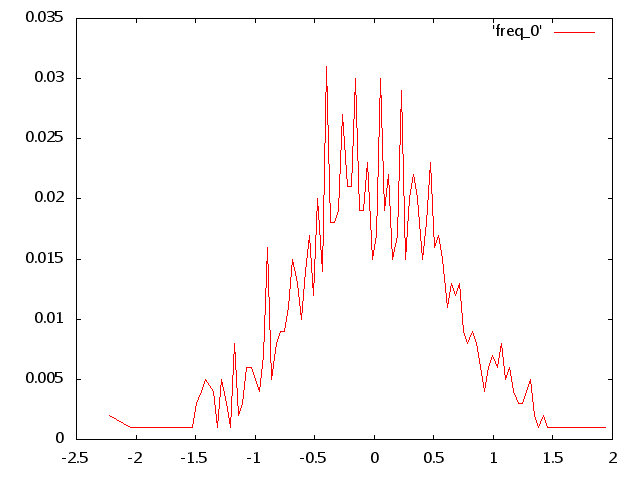
\includegraphics[width=4in]{freq_0.png}
\end{center}

然后把所有粒子的速度设成 $1$, 结果是:
$k=1$ 单位下的温度:
\[
T = \input temp_1
\]
速度分布:
\begin{center}
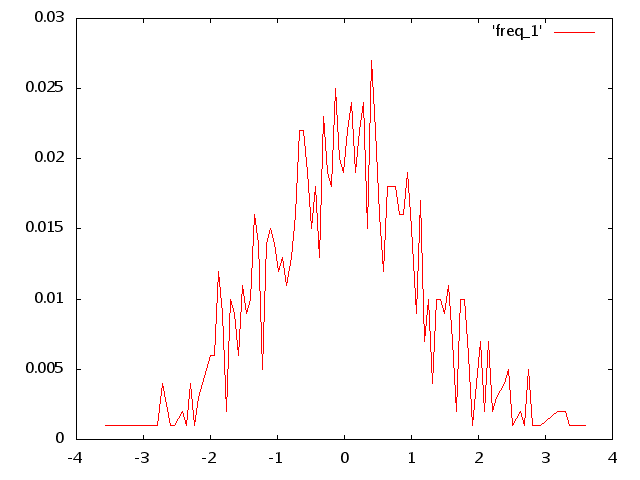
\includegraphics[width=4in]{freq_1.png}
\end{center}

可以看到虽然初始速度是均匀分布的, 模拟结束后粒子的速度分布就变成了Gauss分布.
体系的能量加上 demon 能是守恒的, 因此从最后温度的结果可以看出 demon 能很小,
在 1 的量级. 程序的输出也验证了这一点.
\end{document}